\documentclass[11pt,a4paper]{article}

% Packages
\usepackage[utf8]{inputenc}
\usepackage[T1]{fontenc}
\usepackage{graphicx}
\usepackage{geometry}
\usepackage{amsmath}
\usepackage{booktabs}
\usepackage{float}
\usepackage{caption}
\usepackage{subcaption}
\usepackage{url}
\usepackage{hyperref}
\usepackage{xcolor}

% Page setup
\geometry{
    a4paper,
    left=25mm,
    right=25mm,
    top=30mm,
    bottom=30mm
}
\emergencystretch=2em
\renewcommand{\abstractname}{Sommario}

% Hyperref setup
\hypersetup{
    colorlinks=true,
    linkcolor=blue,
    citecolor=blue,
    urlcolor=blue,
    pdftitle={Suscettibilità agli incendi boschivi su scala stagionale in Alto Adige},
    pdfauthor={Alexandre Dunant},
    pdfsubject={Rapporto tecnico FireScape},
    pdfkeywords={incendi boschivi, Alto Adige, EBM, suscettibilità stagionale}
}

% Title information
\title{\textbf{Suscettibilità agli incendi boschivi su scala stagionale in Alto Adige}\\
\large }

\author{
    Alexandre Dunant --- Progetto FireScape\\
    Eurac Research\\
    Contatto: alexandre.dunant@eurac.edu
}

\date{19 dicembre 2025\\Versione 1.0.0}

\begin{document}

\maketitle

\begin{abstract}
Il presente rapporto descrive un sistema di stima della suscettibilità agli incendi boschivi a risoluzione giornaliera per la Provincia Autonoma di Bolzano (Alto Adige), con una risoluzione spaziale di 250~m. Un modello di base di tipo Explainable Boosting Machine (EBM), addestrato su dati storici di occorrenza degli incendi e privo dell’informazione sui fulmini, è stato applicato alle variabili meteorologiche del periodo 2015--2024. Il modello produce punteggi giornalieri di suscettibilità relativa, che vengono successivamente aggregati per ottenere mappe stagionali. Questi valori non costituiscono probabilità assolute calibrate di incendio. L’approccio consente di conservare la variabilità temporale intrastagionale che viene generalmente persa quando si utilizzano medie climatologiche stagionali.
\end{abstract}

\section{Introduzione}

La presente analisi fornisce stime della suscettibilità stagionale agli incendi boschivi in Alto Adige, derivate da un approccio di modellazione basato su punteggi giornalieri. Invece di calcolare medie climatologiche stagionali e produrre una singola stima per stagione, il sistema genera un punteggio relativo per ciascun giorno del periodo 2015--2024. Tali valori vengono successivamente aggregati per ottenere statistiche stagionali.

Il sistema opera a una risoluzione spaziale di 250~m ed è basato su un modello Explainable Boosting Machine (EBM) di riferimento, addestrato su dati storici di occorrenza degli incendi e su un insieme di variabili ambientali e meteorologiche.

\section{Metodologia}

Il modello utilizzato è un Explainable Boosting Machine (EBM) in configurazione di base, senza l’inclusione dei dati sui fulmini, addestrato su dati di occorrenza degli incendi per il periodo 1999--2024. Le variabili di input includono:

\begin{itemize}
    \item variabili meteorologiche giornaliere (temperatura media giornaliera $T_{\text{daily}}$, precipitazione giornaliera $P_{\text{daily}}$);
    \item indici di siccità (SPEI su scale temporali di 30 e 90 giorni);
    \item caratteristiche topografiche (quota, pendenza, esposizione, componenti nord e est, indice di rugosità del terreno);
    \item caratteristiche della vegetazione (densità di copertura arborea, indice di infiammabilità);
    \item indicatori di accessibilità e pressione antropica (tempo di percorrenza a piedi verso edifici e infrastrutture elettriche, distanza dalla rete stradale);
    \item indicatori temporali (seno e coseno del giorno dell’anno per la codifica stagionale).
\end{itemize}

L’approccio implementato produce un punteggio di suscettibilità per ogni singolo giorno del periodo 2015--2024. I punteggi giornalieri vengono quindi aggregati per stagione al fine di calcolare statistiche riassuntive, quali la media e la deviazione standard.

Il set analitico impiega un disegno presenza--pseudo-assenza: le pseudo-assenze sono campionate e non rappresentano la prevalenza spazio-temporale reale degli incendi. Per questo motivo, l'uscita compresa tra 0 e 1 viene interpretata come indice comparativo di suscettibilità e non come probabilità assoluta. Una probabilità assoluta richiederebbe una calibrazione separata rispetto alla prevalenza osservata.

Le prestazioni del modello sono state valutate mediante una separazione temporale, addestrando il modello sui dati antecedenti al 2020 e testandolo sui dati dal 2020 in poi, al fine di valutare la capacità di generalizzazione su periodi non utilizzati nell'addestramento.

\section{Risultati}

\subsection{Mappe di rischio stagionale}

La Figura~\ref{fig:maps} mostra la distribuzione spaziale della suscettibilità stagionale agli incendi boschivi in Alto Adige, ottenuta aggregando le previsioni giornaliere sull’intero periodo 2015--2024.

\begin{figure}[H]
    \centering
    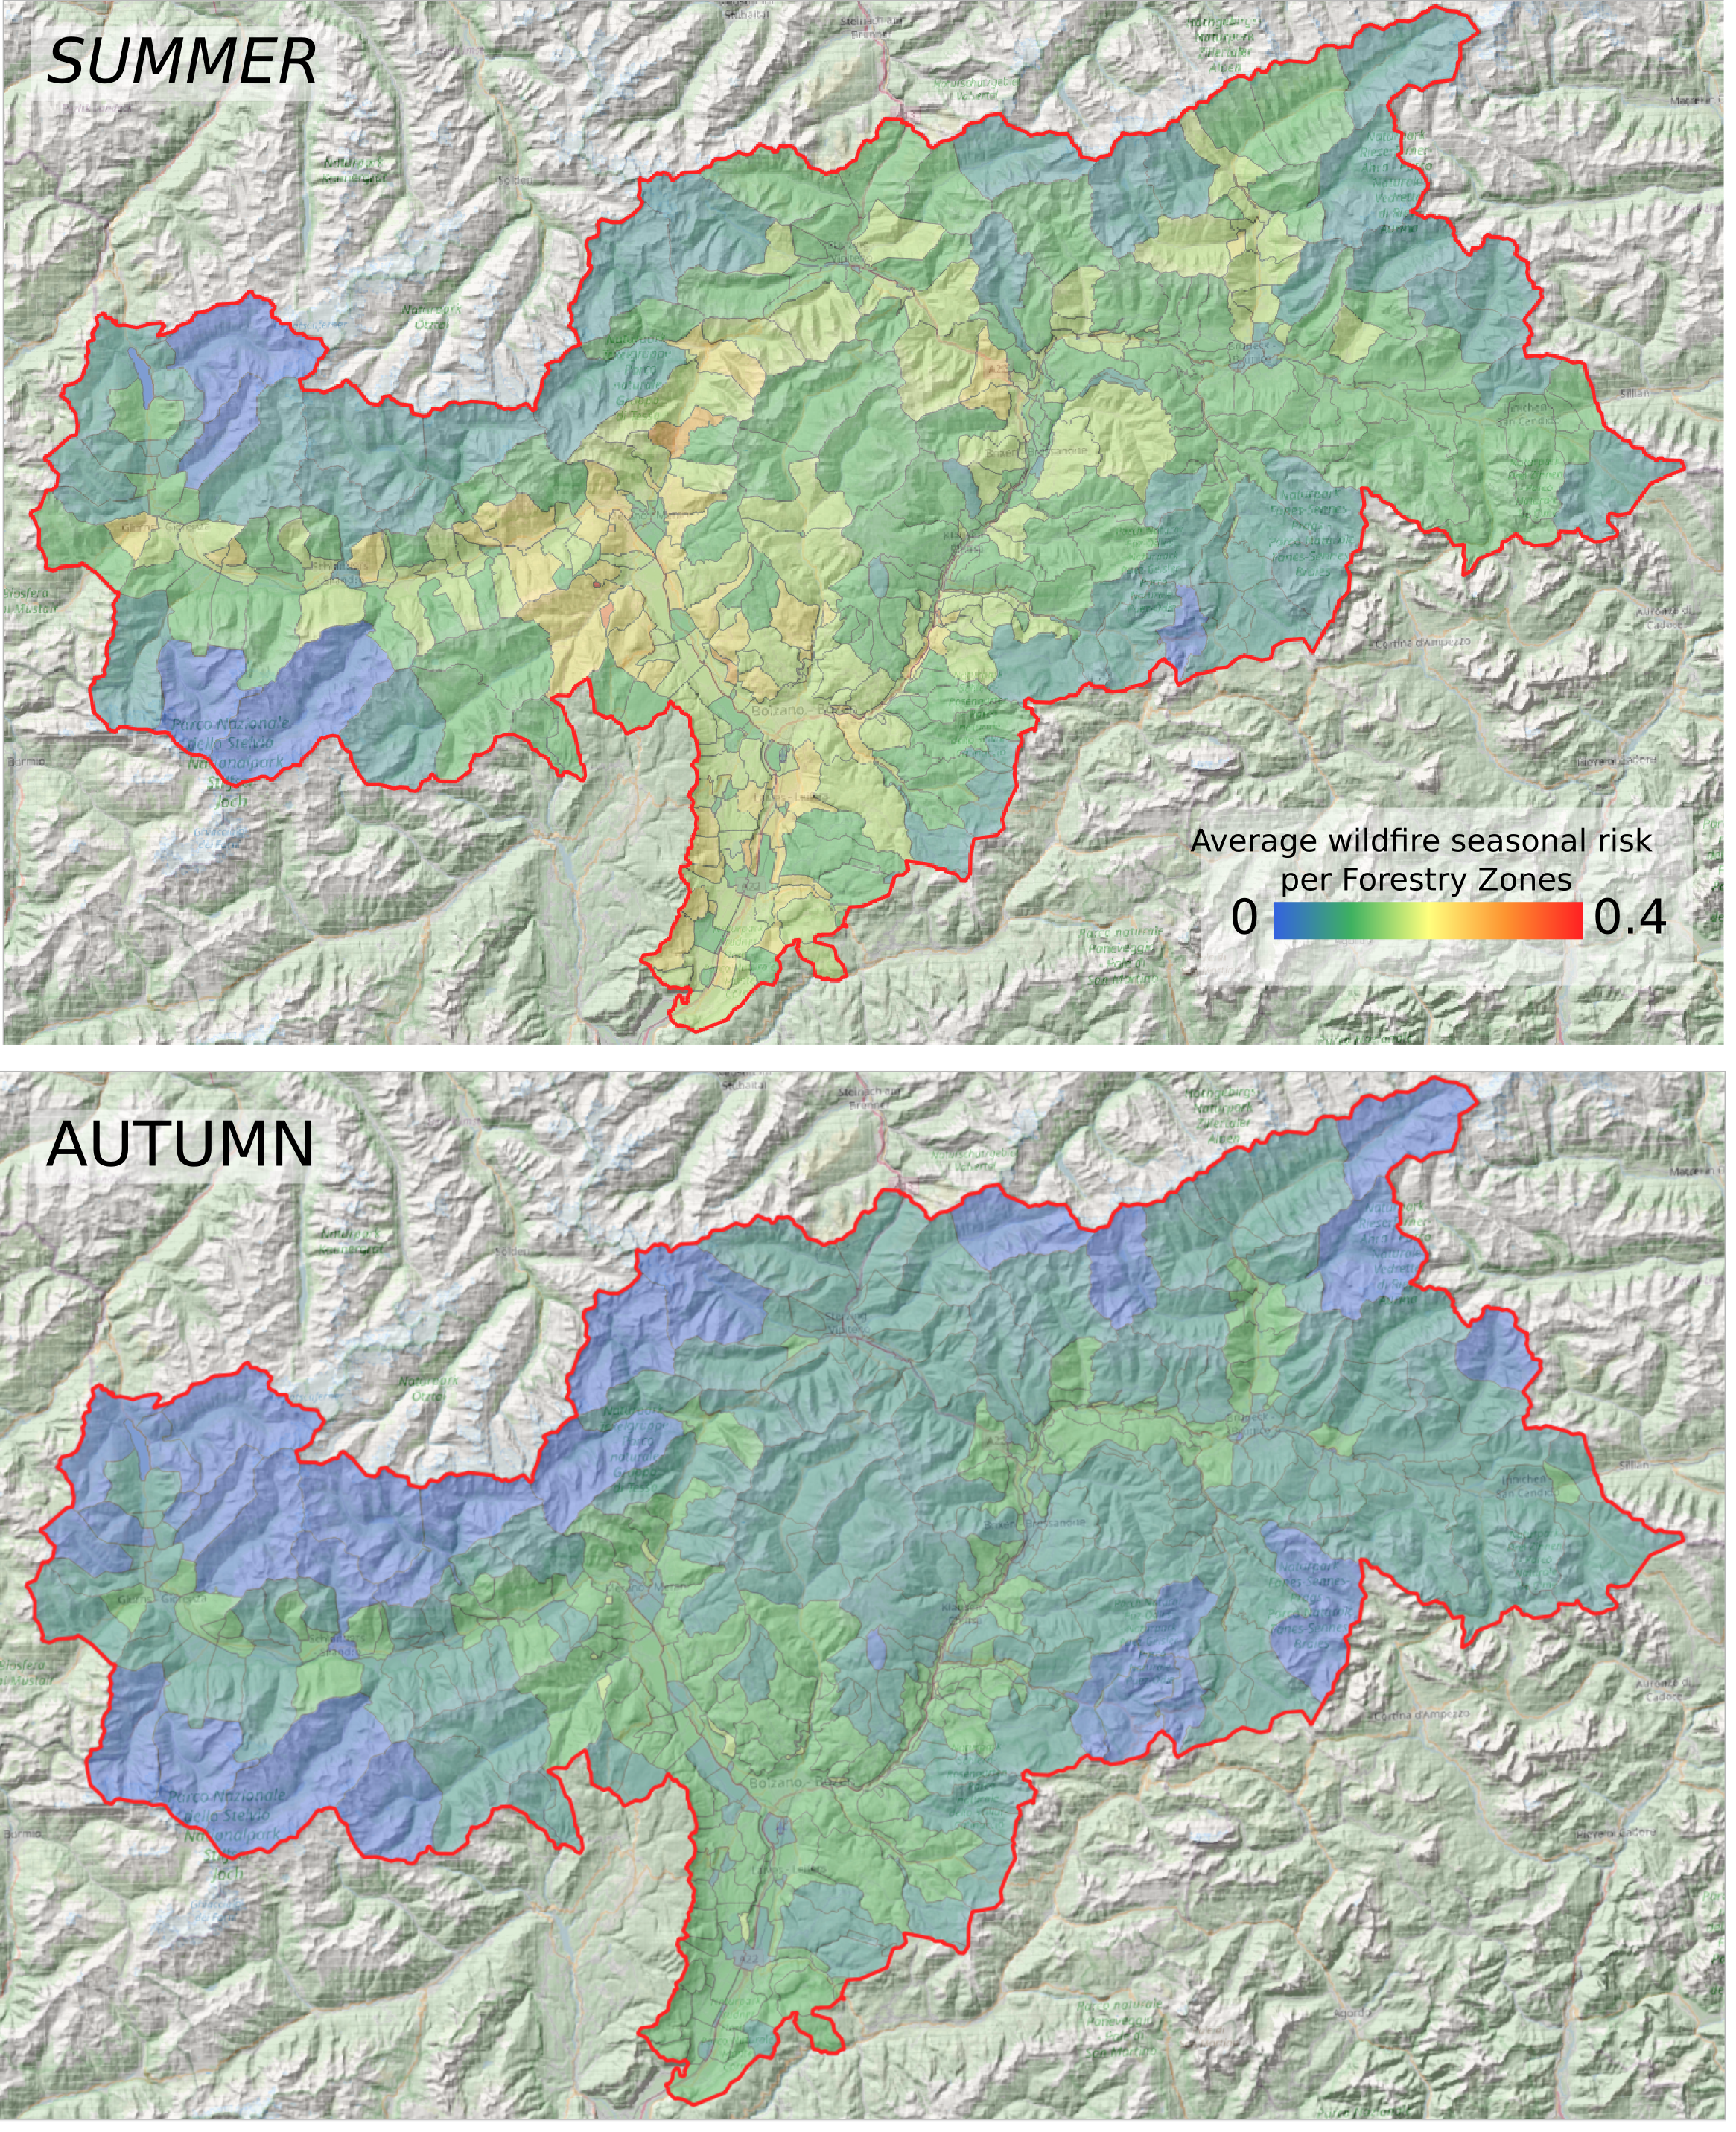
\includegraphics[width=\textwidth]{figures/maps1.png}
\end{figure}
\begin{figure}[H]
    \centering
    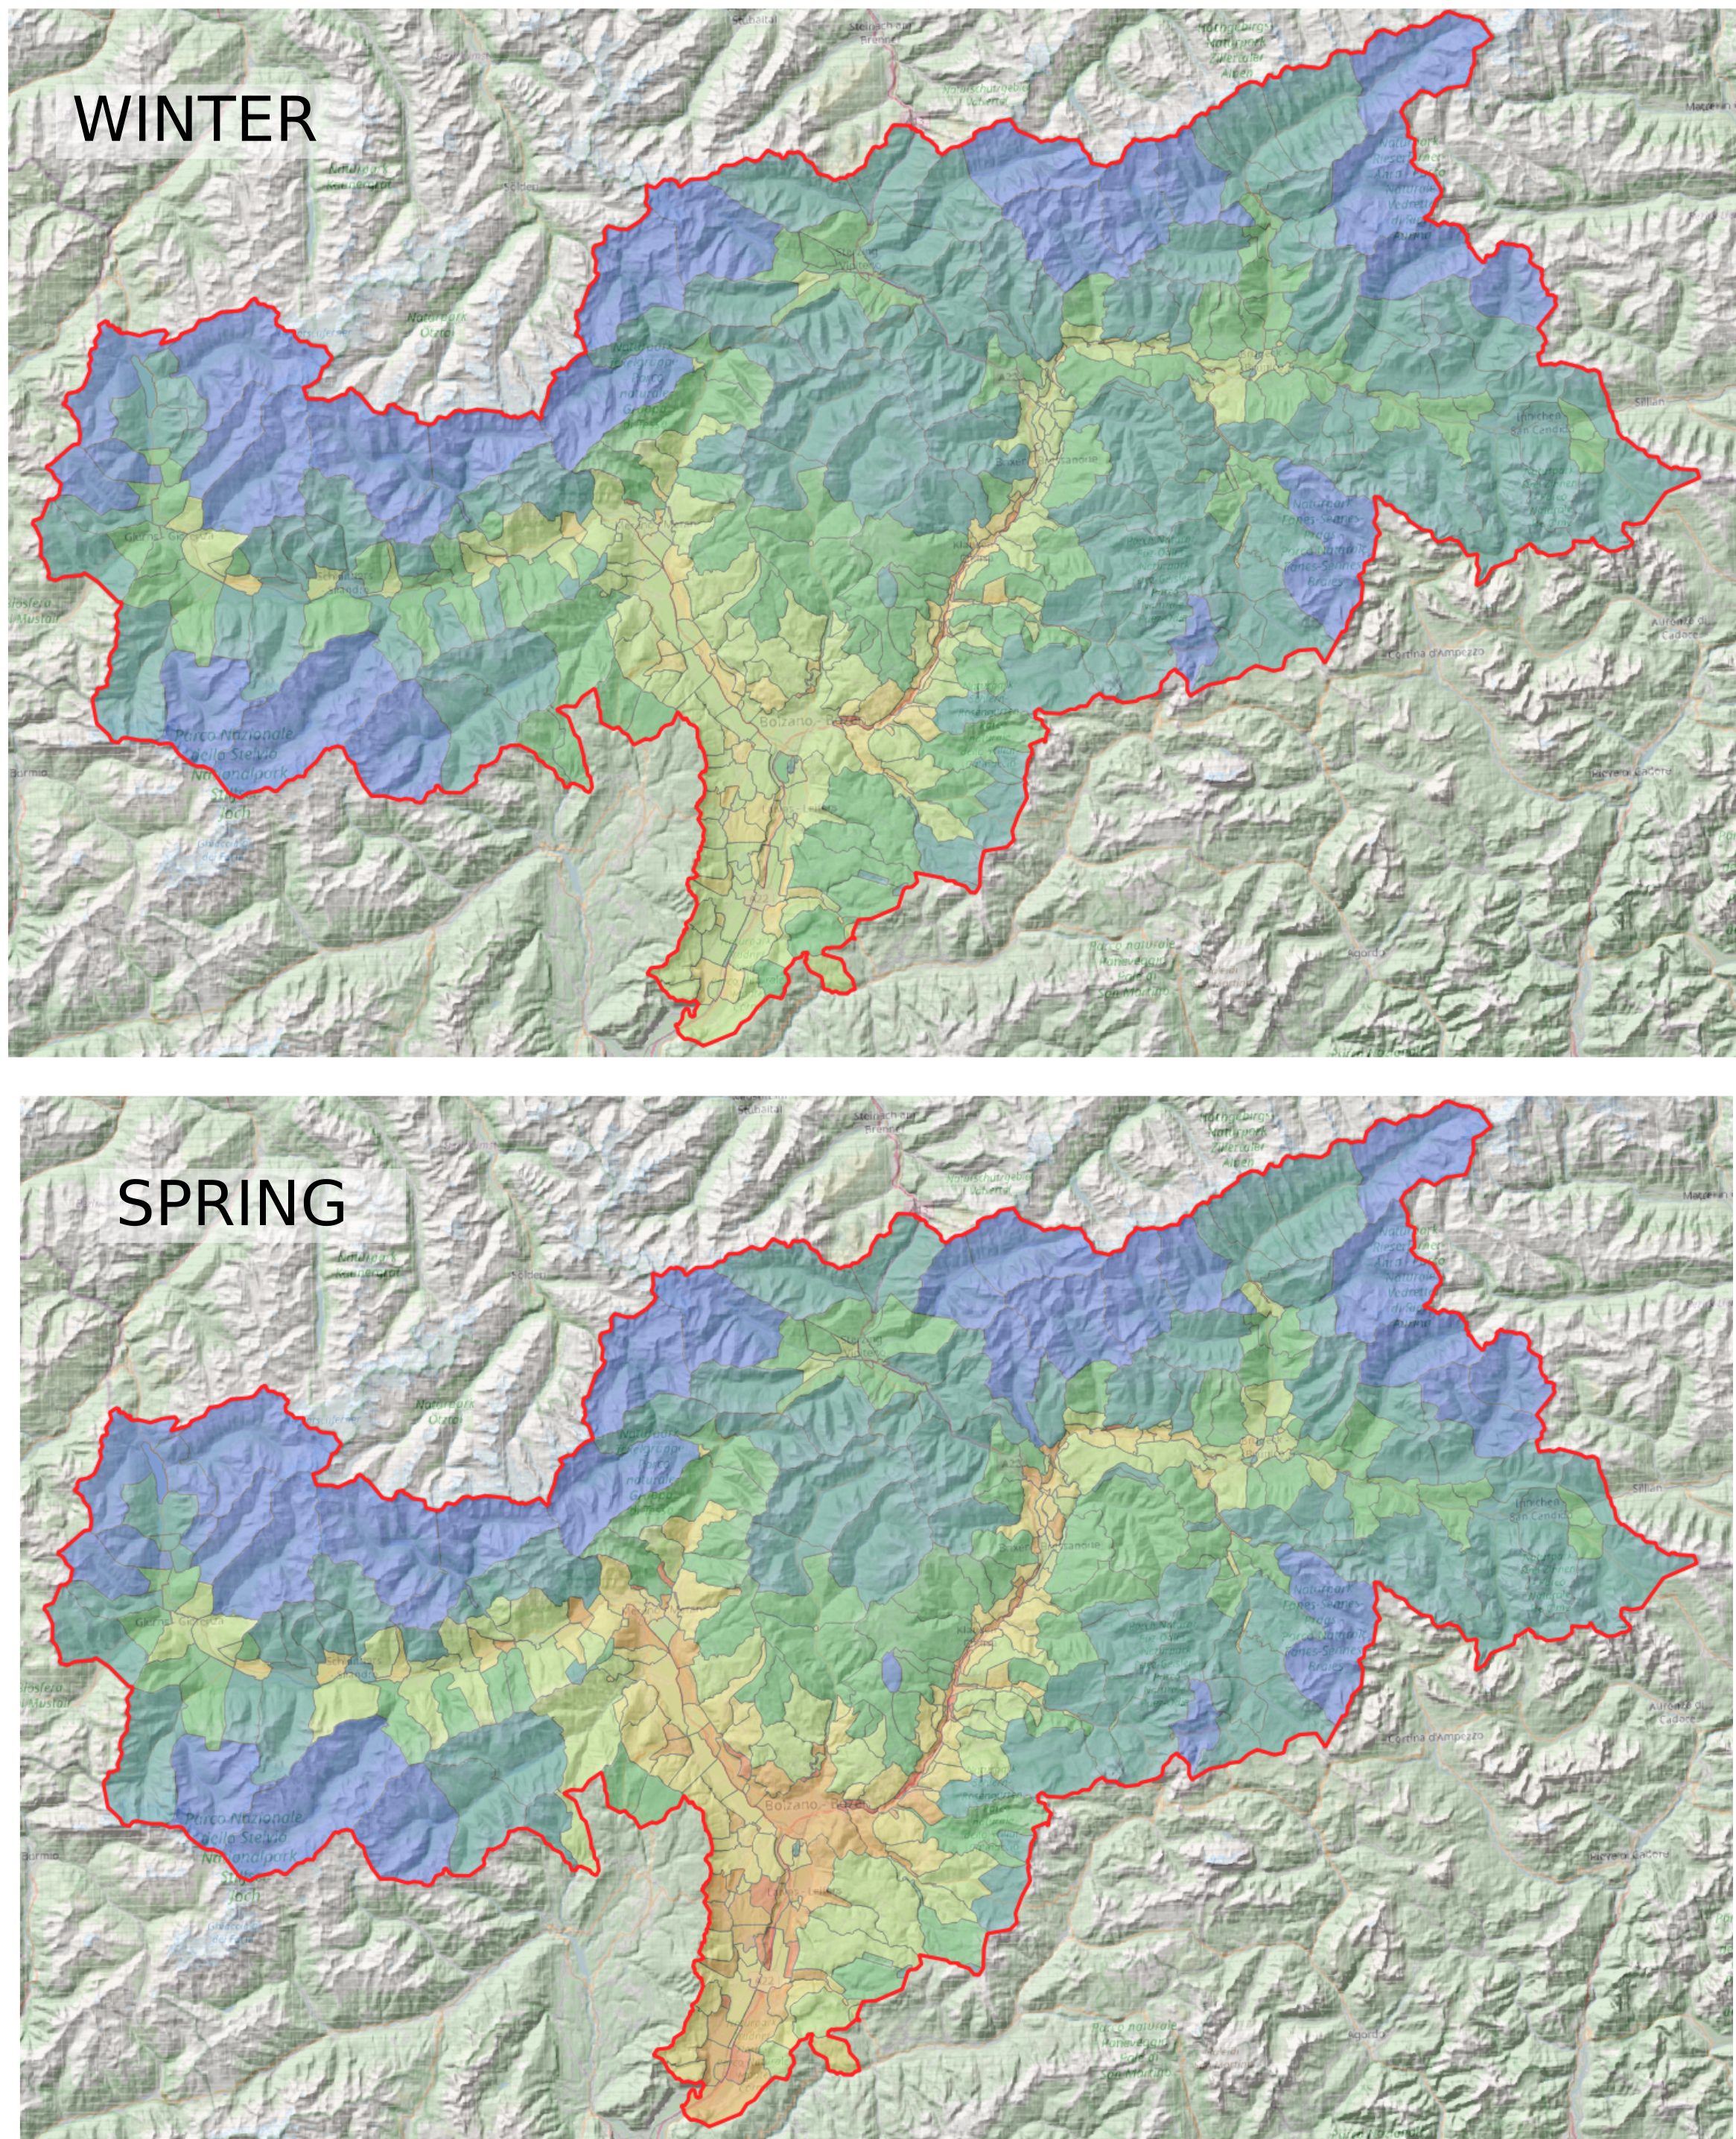
\includegraphics[width=\textwidth]{figures/maps2.png}
    \caption{Mappe stagionali della suscettibilità agli incendi boschivi a risoluzione di 250~m. I valori rappresentano il punteggio EBM medio giornaliero, aggregato su tutti i giorni di ciascuna stagione (2015--2024). Il punteggio è relativo e non è una probabilità assoluta calibrata.}
    \label{fig:maps}
\end{figure}

\subsection{Metriche di prestazione del modello}

La Figura~\ref{fig:metrics} confronta il modello di base utilizzato nel rapporto con una variante sperimentale che include i fulmini. Le metriche sono calcolate sul campione presenza--pseudo-assenza; AUC-PR, accuratezza e Brier score dipendono quindi dal disegno di campionamento e non descrivono direttamente le prestazioni alla prevalenza reale.

\begin{figure}[H]
    \centering
    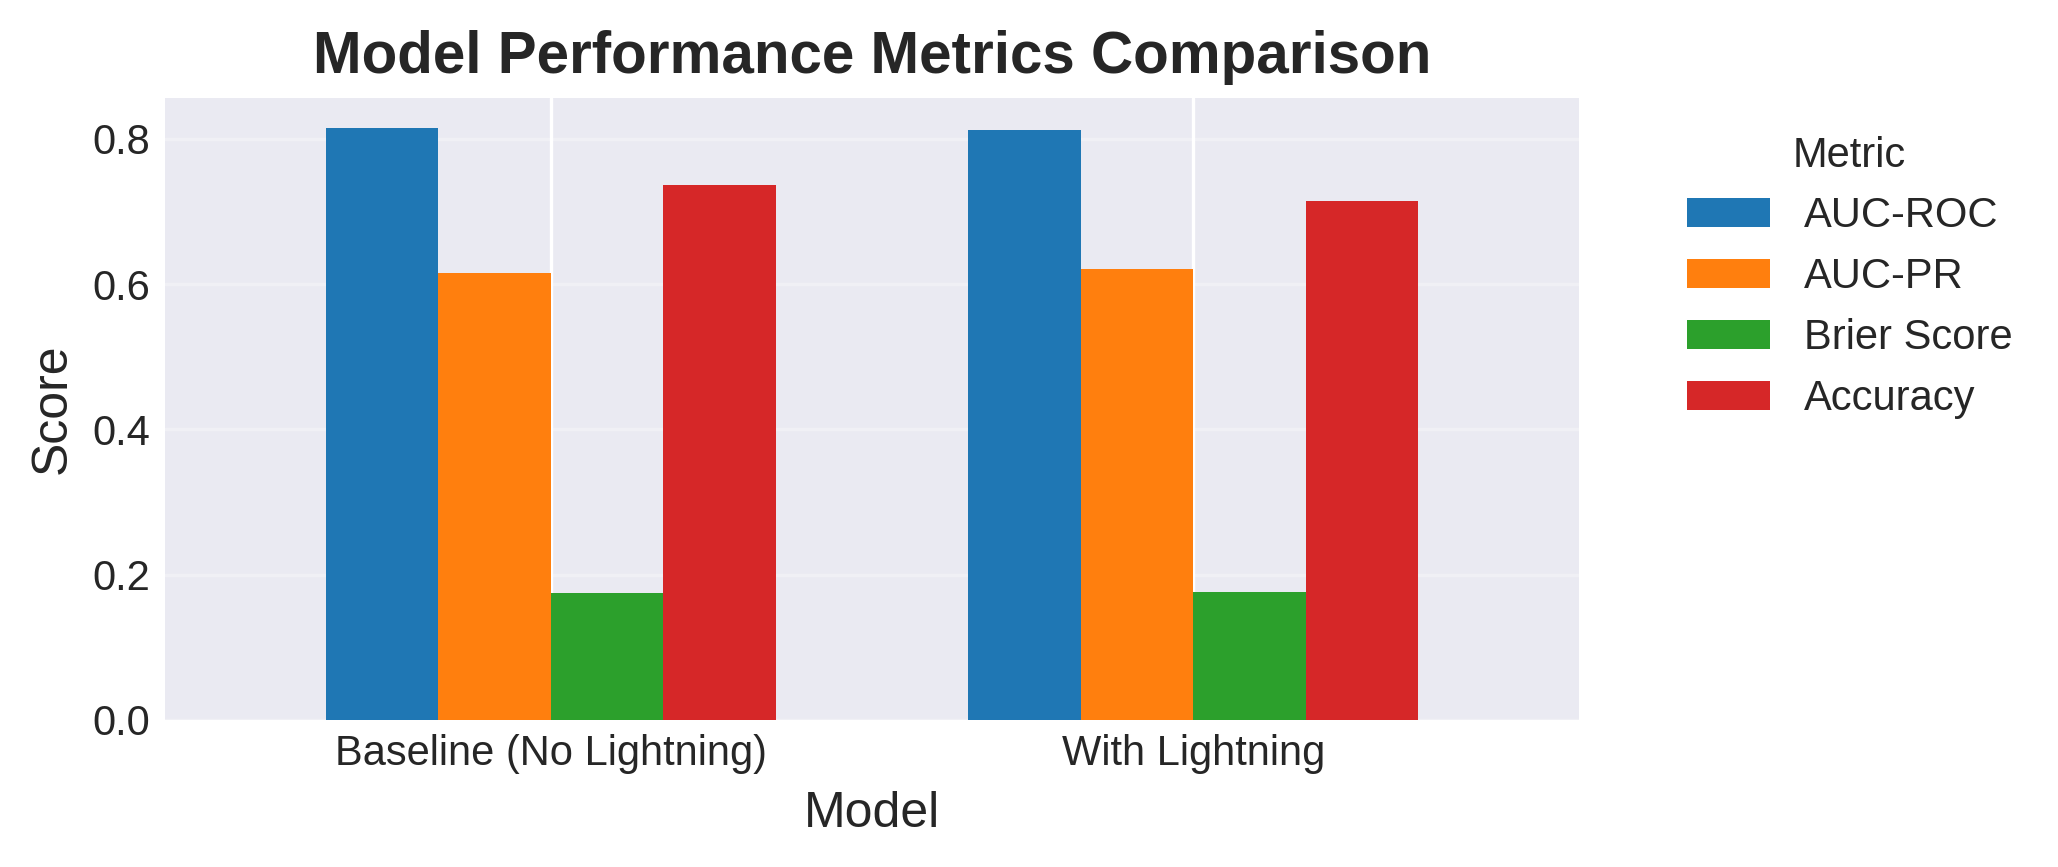
\includegraphics[width=0.85\textwidth]{figures/model_comparison_metrics.png}
    \caption{Confronto descrittivo delle metriche per il modello di base senza fulmini e la variante con fulmini, valutati sui rispettivi campioni. I periodi disponibili differiscono e i valori non costituiscono una verifica di calibrazione sulla prevalenza reale.}
    \label{fig:metrics}
\end{figure}

L’utilizzo di un modello EBM, classificabile come \emph{glass model}, consente una chiara interpretazione dei fattori che influenzano le previsioni del modello (Figura~\ref{fig:f_importance}). È importante notare che l’inclusione dei dati sui fulmini nel set di addestramento modifica in modo significativo l’importanza relativa delle variabili e richiede pertanto un’analisi dedicata in studi futuri.

\begin{figure}[H]
    \centering
    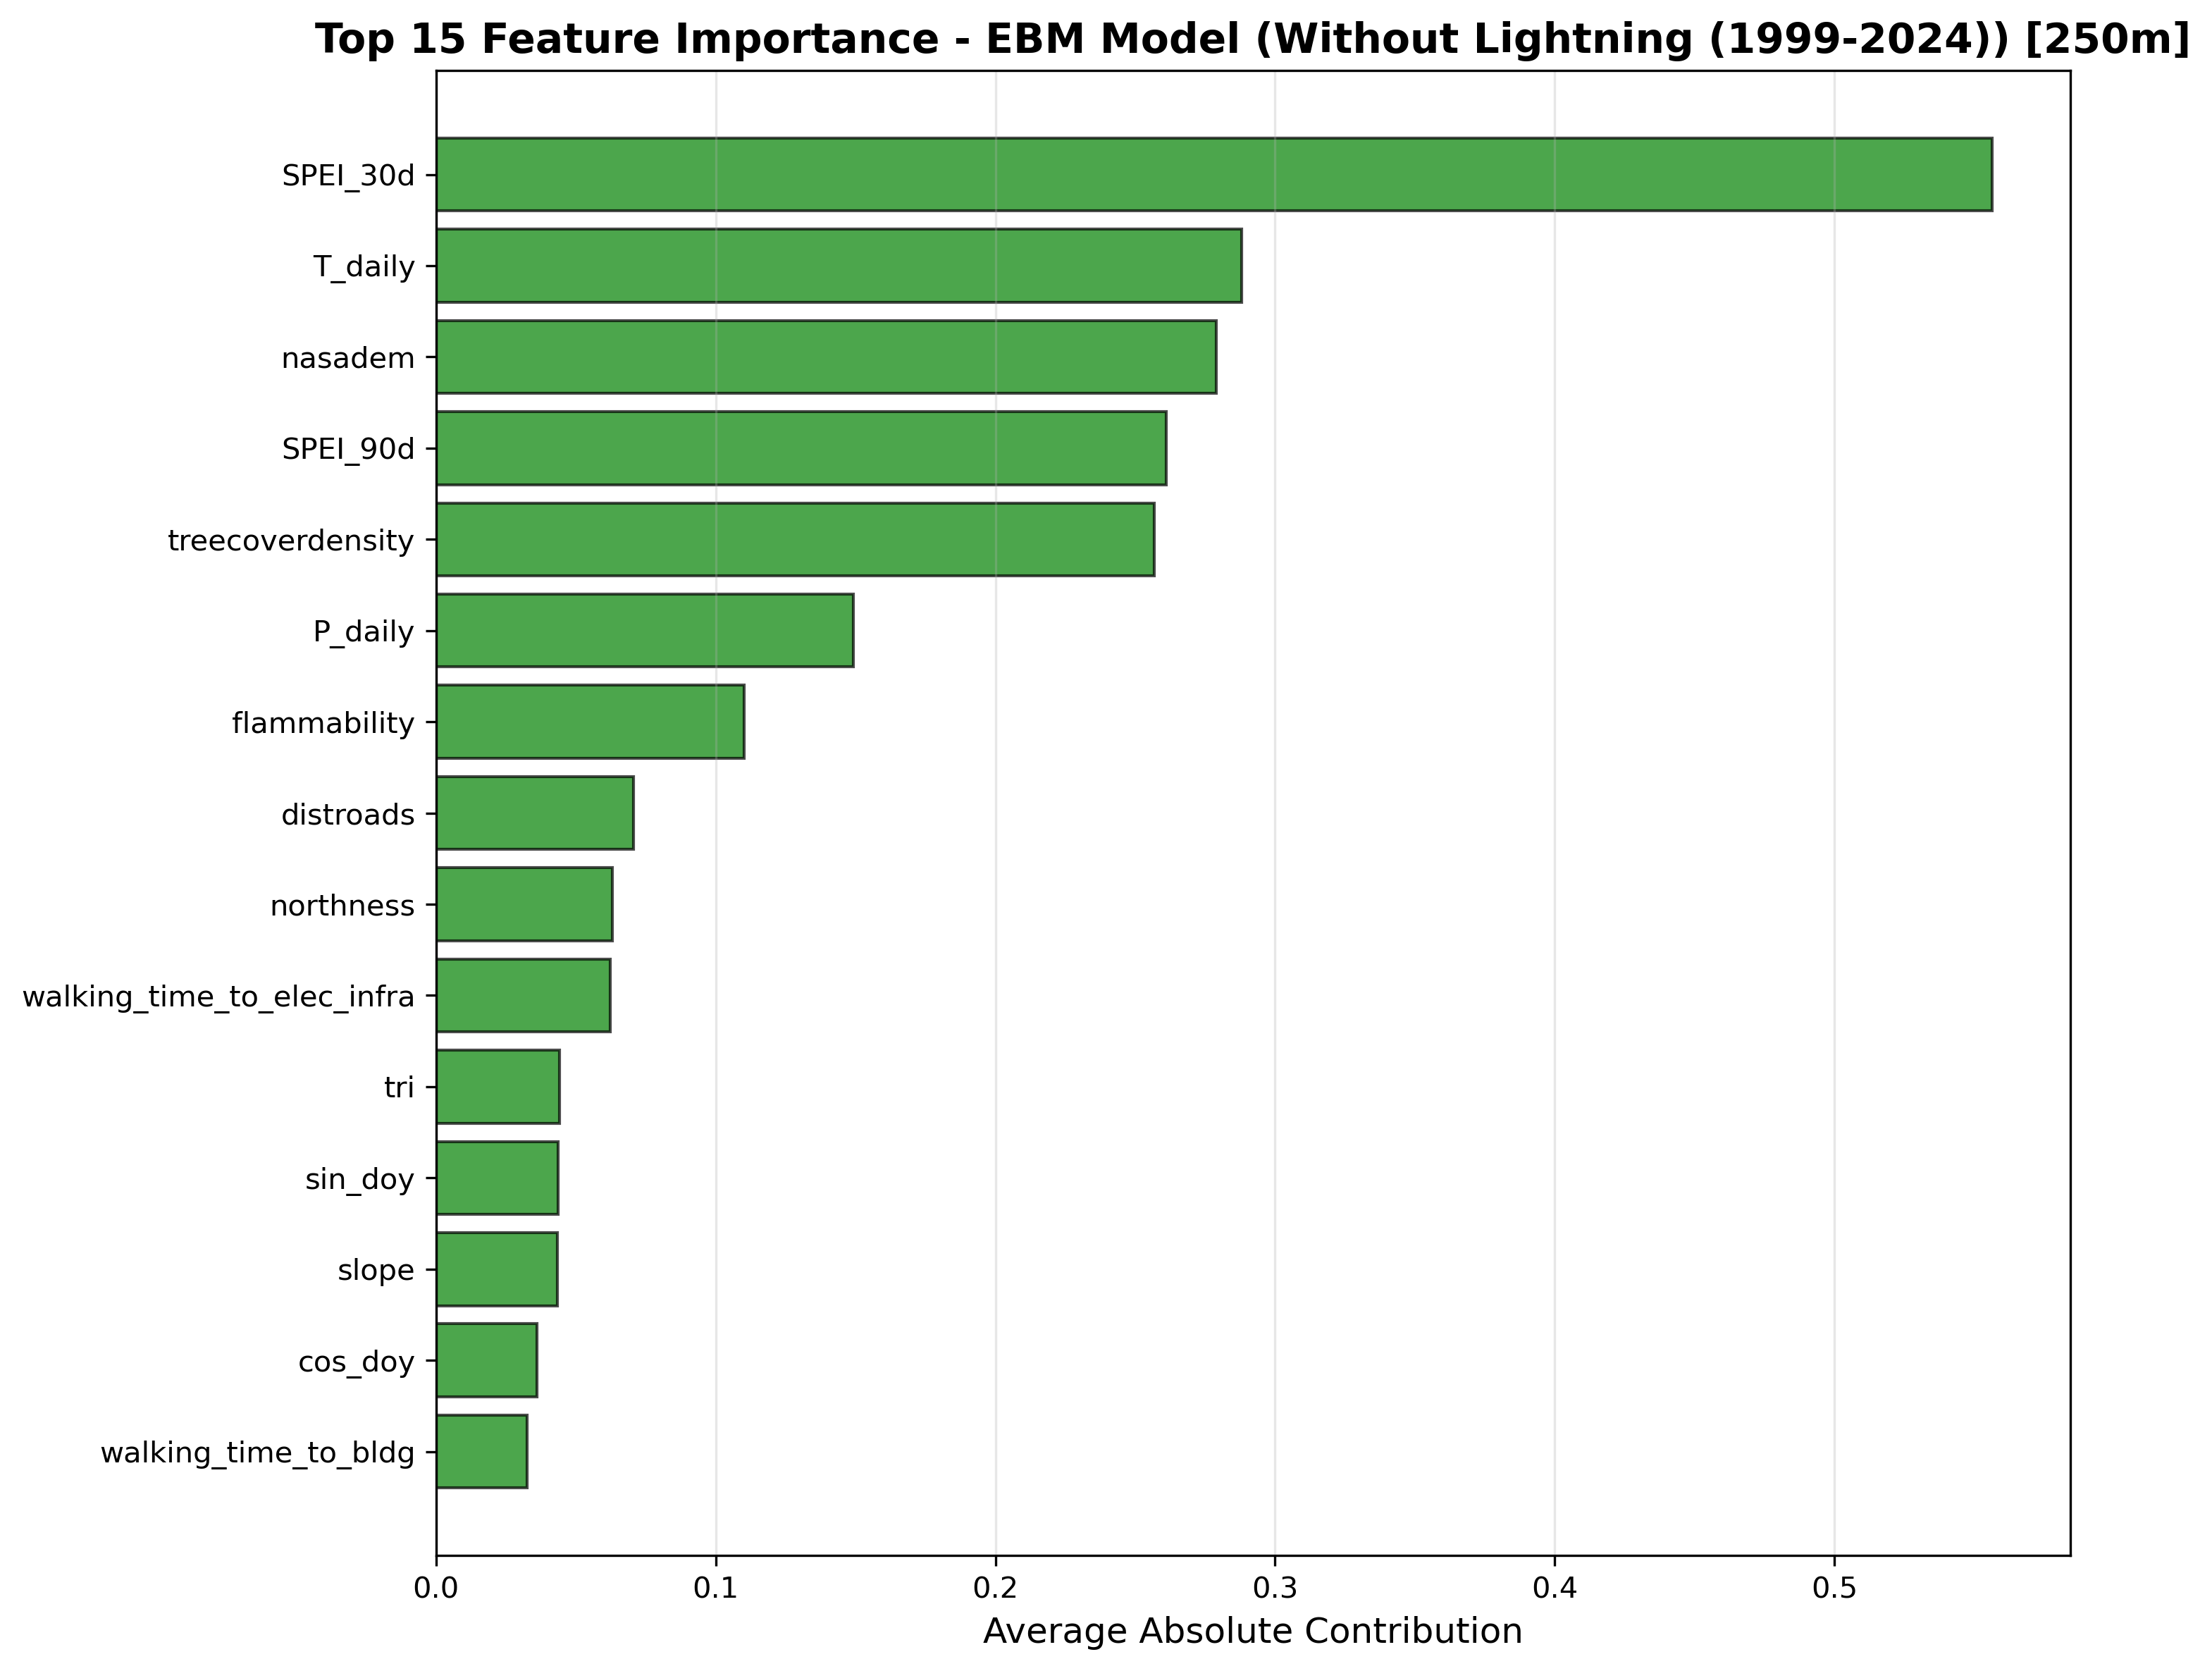
\includegraphics[width=1\linewidth]{figures/feature_importance.png}
    \caption{Classifica dell’importanza delle variabili per il modello EBM presentato}
    \label{fig:f_importance}
\end{figure}

\section{Limiti di interpretazione}

Le mappe descrivono differenze relative di suscettibilità secondo il modello e i dati disponibili; non stimano direttamente il numero atteso di incendi né la probabilità assoluta di un incendio in una cella e in un giorno. Le metriche precision-recall dipendono inoltre dalla proporzione di presenze e pseudo-assenze nel campione di valutazione. La separazione temporale misura la trasferibilità interna verso anni successivi, ma non sostituisce una validazione esterna su un inventario indipendente. Le importanze delle variabili descrivono il contributo del modello predittivo e non dimostrano rapporti causali. Infine, alcuni dati provinciali e meteorologici non sono redistribuiti nel pacchetto pubblico per vincoli di accesso e licenza, limitando la riproducibilità completa da parte di terzi.

\section{Specifiche tecniche}

\begin{table}[H]
\centering
\caption{Specifiche del sistema e caratteristiche dei dati}
\label{tab:specs}
\begin{tabular}{ll}
\toprule
\textbf{Parametro} & \textbf{Valore} \\
\midrule
Risoluzione spaziale & 250 m $\times$ 250 m \\
Periodo di addestramento del modello & 1999--2024 (26 anni) \\
Periodo di previsione & 2015--2024 (10 anni) \\
Previsioni giornaliere & $\sim$3.650 giorni $\times$ griglia spaziale \\
Area di studio & Provincia Autonoma di Bolzano (Alto Adige) \\
Tipologia di modello & EBM di base (senza fulmini) \\
Approccio di validazione & Separazione temporale (test dal 2020) \\
Formato di output & Indice relativo di suscettibilità (0--1) \\
\bottomrule
\end{tabular}
\end{table}

\end{document}
